\documentclass[a4paper,12pt]{article}
\usepackage[utf8]{inputenc}
\usepackage[T1]{fontenc}
\usepackage[brazil]{babel}
\usepackage{geometry}
\geometry{
    left=2cm,
    right=2cm,
    top=2cm,
    bottom=2cm
}
\usepackage{setspace}
\setstretch{1.0}
\usepackage{graphicx, xcolor, comment, enumerate, multirow, multicol}
\usepackage{indentfirst}
\usepackage{amsmath, amsthm, amsfonts, amssymb, dsfont, mathtools}
\usepackage{caption, subcaption}
\captionsetup[figure]{labelfont=bf}
\usepackage{times}
\usepackage{booktabs}
\usepackage{float}
\usepackage{url}
\usepackage{hyperref}
\usepackage{appendix}
\usepackage{listings}

\usepackage{listings}
\usepackage{xcolor}

\definecolor{codegray}{rgb}{0.5,0.5,0.5}
\definecolor{codepurple}{rgb}{0.58,0,0.82}
\definecolor{backcolor}{rgb}{0.95,0.95,0.92}

\lstdefinestyle{pythonstyle}{
    backgroundcolor=\color{backcolor},   
    commentstyle=\color{codegray},
    keywordstyle=\color{blue},
    numberstyle=\tiny\color{codegray},
    stringstyle=\color{codepurple},
    basicstyle=\ttfamily\footnotesize,
    breaklines=true,
    captionpos=b,
    keepspaces=true,
    numbers=left,
    numbersep=5pt,
    showspaces=false,
    showstringspaces=false,
    showtabs=false,
    tabsize=4,
    language=Python
}

\lstset{style=pythonstyle}


% ----------------------------------------------------------
% Início do documento
% ----------------------------------------------------------

\begin{document}

\begin{center}
    \LARGE{\bf Controle da Planta Hidraúlica LabVolt 3502} \\
    \vspace{0.2cm}
    \large{
        Carlos Eduardo Luyo Gonçalves$^1$,
        Eduardo De Paiva Martins Filho$^2$,
        Guilherme Machado Ribeiro França$^3$,
        Victor de Melo Lima Evangelista$^4$,
        Welliton Borges Araújo$^5$
    } \\
    \vspace{0.25cm}
    \small{
        Matrícula: 20231003800255$^1$ \\
        Matrícula: 20231003800042$^2$ \\
        Matrícula: 20232003800040$^3$ \\
        Matrícula: 20232003800032$^4$ \\
        Matrícula: 20222003800060$^5$
    }
\end{center}

\hrulefill

\begin{abstract}
    Neste relatório reporta-se a atividade desenvolvida na disciplina ELT1119 \textbf{Redes e Aplicações IOT}, pelos discentes da PUC, que consiste em utilizar a ESP32 para controlar a planta hidraúlica por meio do protocolo MQTT integrado a plataforma NodeRED.  \\

    \textbf{Palavras-chave}: NodeRED, MQTT, ESP32.
\end{abstract}
\section{Introdução}
\par Nesse relatório reporta-se a atividade desenvolvida, na disciplina ENG1119 Redes e Aplicações IOT, pelos discentes da PUC que consiste em controlar uma variável de processo, vazão, da
Estação de Fluxo LabVolt Modelo 3502 presente nos laboratórios da instituição de ensino superior. O controle será feito pela utilização de um  broker remoto hospedado em \textbf{test.mosquitto.org}. O protocolo de comunicação utilizado será o MQTT, que é um protocolo leve de mensagens, ideal para aplicações de Internet das Coisas (IoT). A plataforma NodeRED será utilizada para criar a interface gráfica do usuário (GUI) e integrar o ESP32 com o broker MQTT. O ESP32 atuará como um dispositivo IoT, enviando e recebendo dados do broker MQTT. A comunicação entre o ESP32 e o broker será feita por meio de uma conexão Wi-Fi. A principal diferença do projeto atual para o passado é o protocolo a ser utilizado. Anteriormente se usava o protocolo HTTP, sigla para Hypertext Transfer Protocol, que é um protocolo de comunicação utilizado na transferência de dados na web. O HTTP é um protocolo baseado em requisições e respostas, onde o cliente envia uma requisição ao servidor e o servidor responde com os dados solicitados. No entanto, o HTTP não é ideal para aplicações de IoT, pois é um protocolo pesado e consome muitos recursos. O MQTT, por outro lado, é um protocolo leve e eficiente, ideal para aplicações de IoT. Ele permite a comunicação entre dispositivos de forma rápida e eficiente, consumindo poucos recursos. Além disso, o MQTT é baseado em tópicos, onde os dispositivos publicam e assinam tópicos para enviar e receber dados. Isso permite uma comunicação mais eficiente entre os dispositivos, pois os dados são enviados apenas quando necessário, reduzindo o consumo de largura de banda e energia. \\
Neste experimento, o controle da planta será feito por uma interface web hospedada no ESP32. O
valor ajustado pelo usuário (via slider) será convertido em sinal analógico através do pino DAC, que
é conectado ao terminal de entrada analógica do inversor de frequência da planta didática de vazão
modelo 3502. A página web exibirá em tempo real:
\begin{itemize}
    \item O valor DAC (0 a 255).
    \item Frequência aplicada (0 a 60 Hz).
    \item A vazão estimda (0 a 38 LPM).
\end{itemize}
\begin{figure}[H]
    \centering
    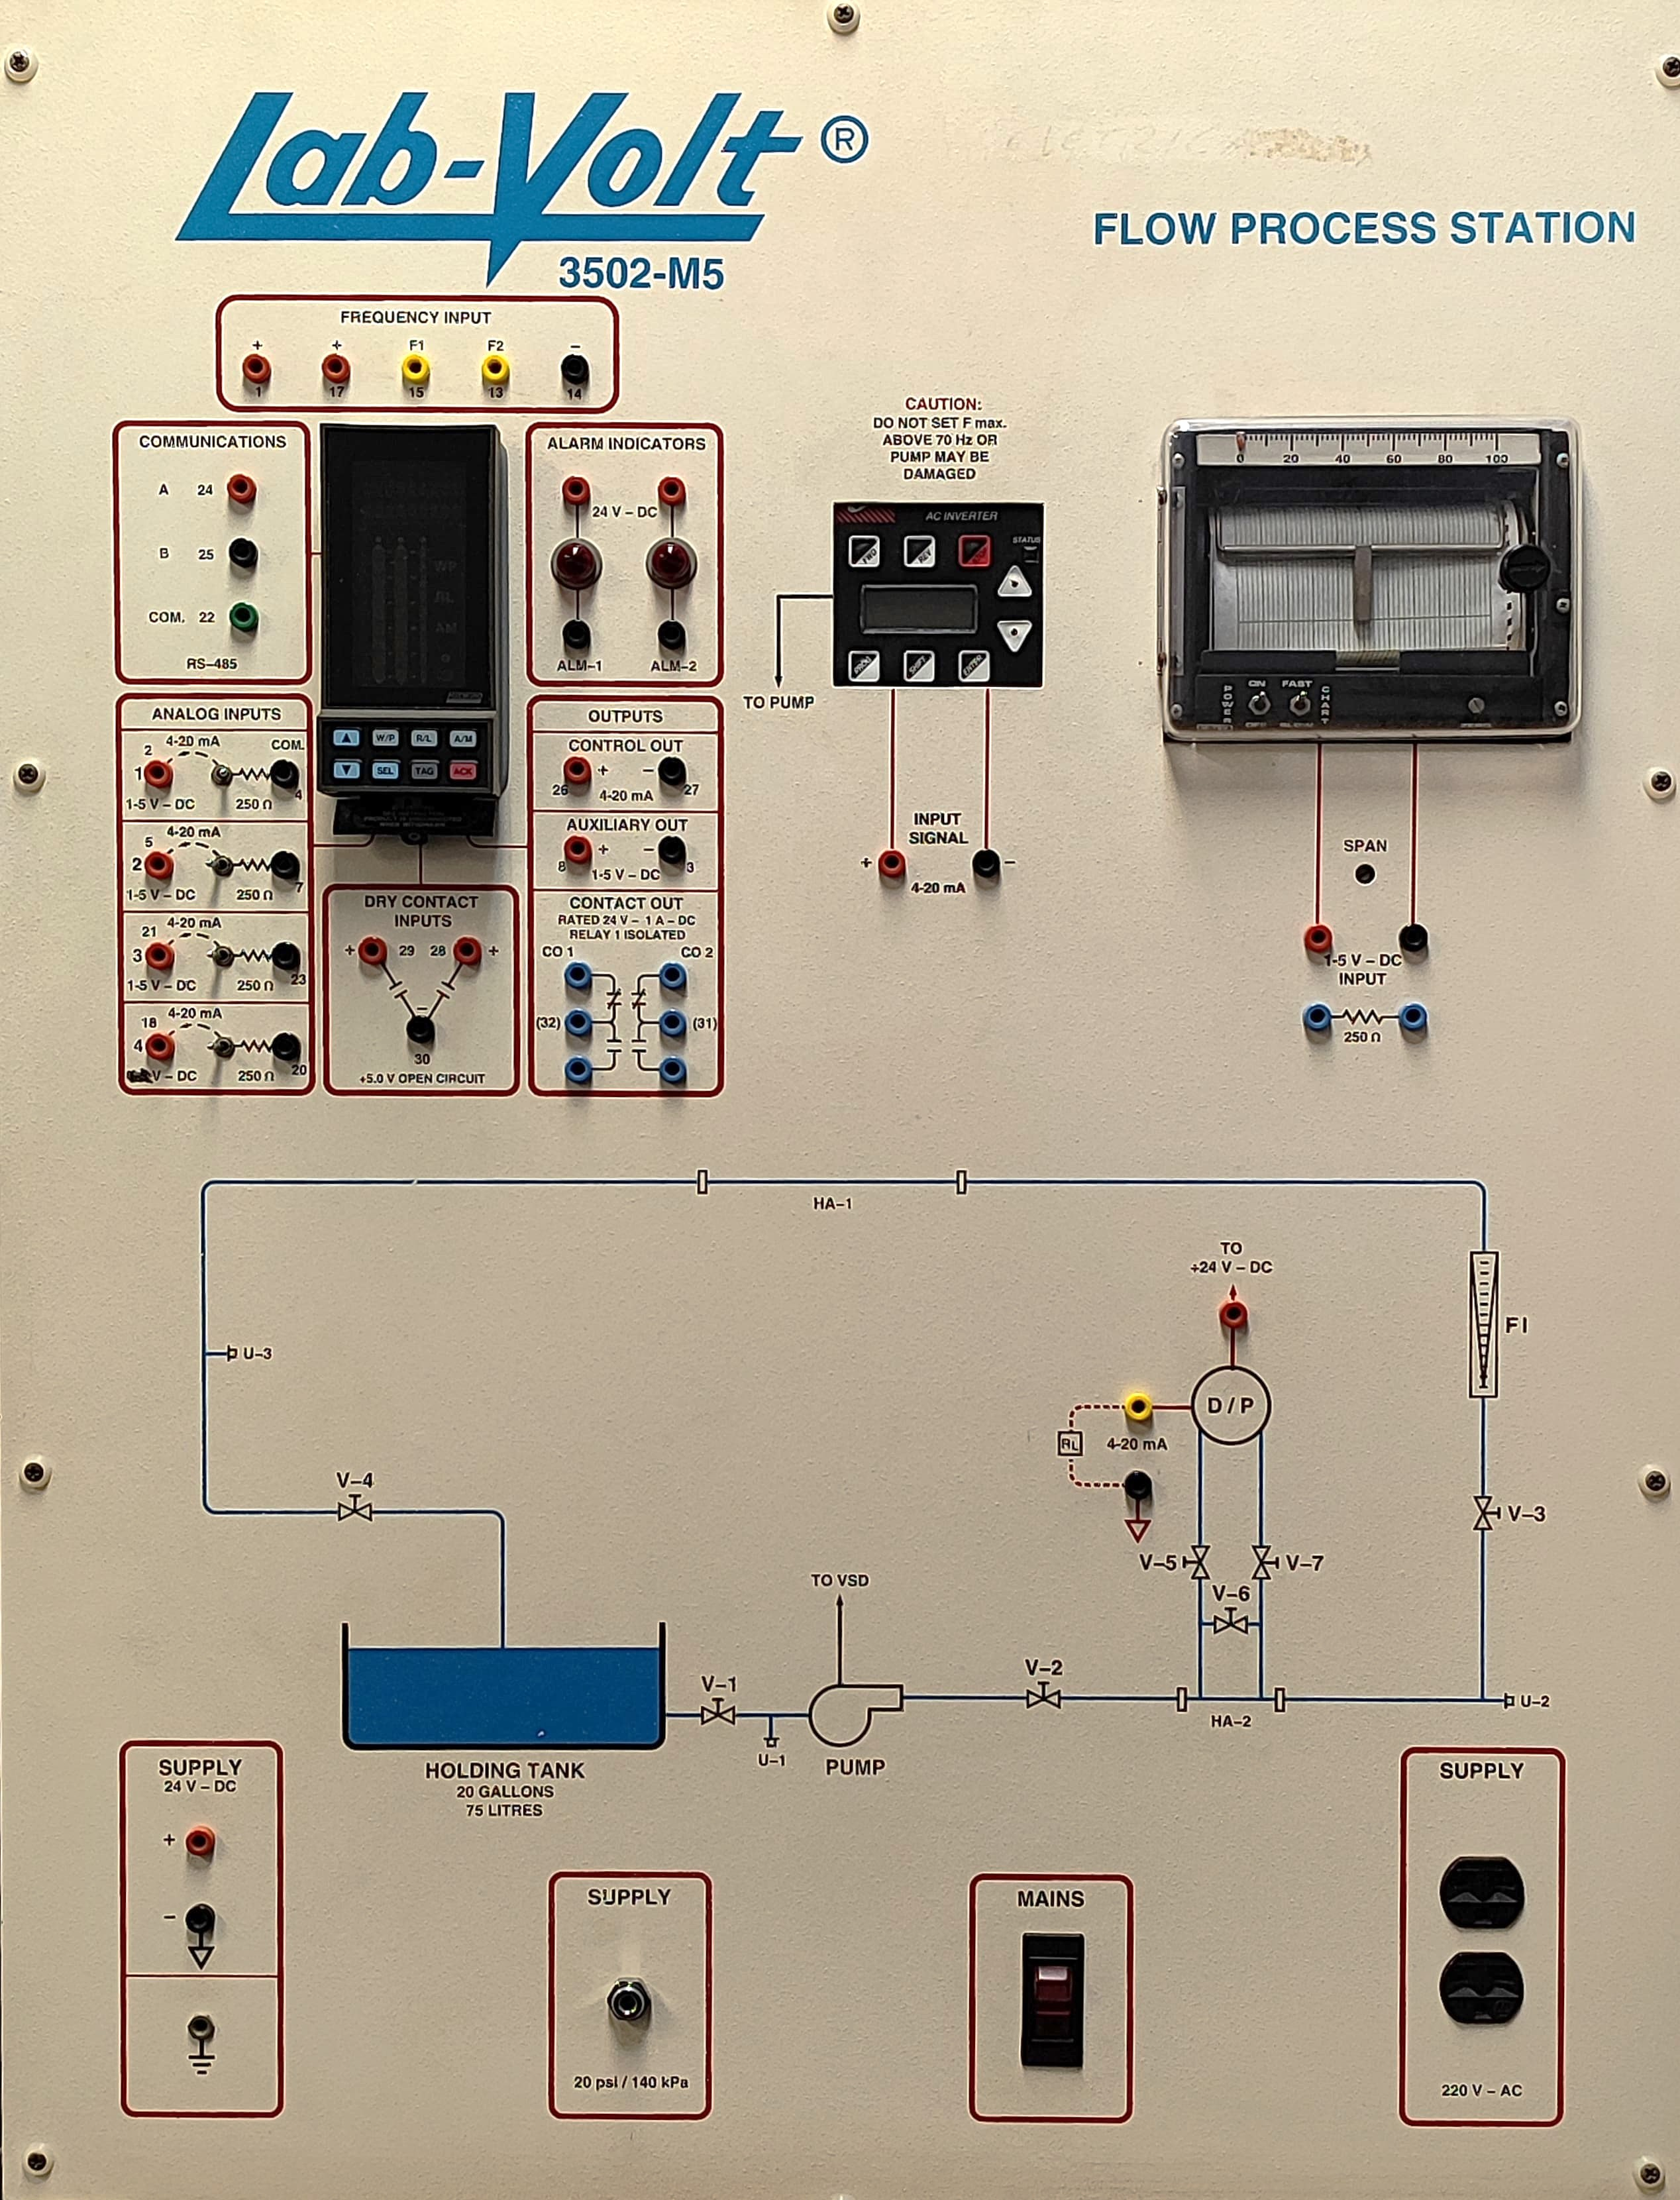
\includegraphics[width=0.5\textwidth]{Figuras/planta.jpeg}
    \caption{Modelo de Planta Hidráulica LabVolt 3502.}
    \label{fig:planta}
\end{figure}

\section{Procedimentos Experimentais}
\par Para o desenvolvimento do projeto, foram utilizados os seguintes componentes:
\begin{itemize}
    \item \textbf{Planta Hidráulica LabVolt 3502}: equipamento utilizado para simular um sistema hidráulico, permitindo o controle da vazão de água.
    \item \textbf{ESP32}: microcontrolador utilizado para controlar a planta hidráulica e se comunicar com o broker MQTT.
    \item \textbf{NodeRED}: plataforma de desenvolvimento de aplicações IoT, utilizada para criar a interface gráfica do usuário (GUI) e integrar o ESP32 com o broker MQTT.
    \item \textbf{Broker MQTT}: serviço de mensagens utilizado para enviar e receber dados entre o ESP32 e a plataforma NodeRED. Neste projeto, foi utilizado o broker remoto \textbf{test.mosquitto.org}.
    \item \textbf{Circuito pra Transformar Tensão em Corrente}: circuito utilizado para transformar a tensão medida pelo sensor de pressão em uma corrente proporcional.
    \item \textbf{Circuito pra Transformar Corrente em Tensão}: circuito utilizado para transformar a corrente medida pelo sensor de pressão em uma tensão proporcional.
\end{itemize}

\subsection{Código do ESP32}

O código do ESP32 foi desenvolvido em linguagem MicroPython e é o seguinte:
\begin{lstlisting}[language=Python, caption={Código Principal do ESP32}, label={lst:codigoESP32}]
import network
import time
from utime import sleep
from machine import Pin, DAC, ADC
from umqtt.simple import MQTTClient
import machine

# ==== CONFIGURAÇÕES ====#
SSID = 'Aegis2.4GHz'
SENHA = 'Strudel#22'
BROKER = 'test.mosquitto.org'

TOPICO_VAZAO = b'esp32/VAZAO'
TOPICO_VAZAO_RESPOSTA = b'esp32/VAZAO/RESPOSTA'
TOPICO_VAZAO_CORRENTE = b'esp32/VAZAO/CORRENTE'
TOPICO_DAC = b'esp32/DAC'
TOPICO_DAC_FREQ = b'esp32/DAC/FREQ'
TOPICO_DAC_CORRENTE_FREQ = b'esp32/DAC/CORRENTE/FREQ'

# ==== CONFIGURAÇÕES ====#

ENVIAR_PERIODICAMENTE = False
INTERVALO_ENVIO_MS = 2000
DEBUG = True

# ==== HARDWARE ====#
adc = ADC(Pin(32))
adc.atten(ADC.ATTN_11DB)
dac = DAC(Pin(25))
dac.write(0)

# ==== VARIÁVEIS ====#
vazao = 0.0
limiar_adc = 1200
ultimo_envio = time.ticks_ms()

# ==== CONEXÃO WIFI ==== #
wifi = network.WLAN(network.STA_IF)
wifi.active(True)
wifi.connect(SSID, SENHA)

tentativas = 0
while not wifi.isconnected() and tentativas < 10:
    if DEBUG:
        print("Conectando ao Wi-Fi...")
    time.sleep(1)
    tentativas += 1

if not wifi.isconnected():
    print("Falha ao conectar Wi-Fi. Reiniciando...")
    machine.reset()

print("Wi-Fi conectado com IP:", wifi.ifconfig()[0])

# ==== FUNÇÕES AUXILIARES ==== #

def atualizar_vazao():
    leitura_adc = adc.read()
    if leitura_adc >= limiar_adc:
        return (38 / (4095 - limiar_adc)) * (leitura_adc - limiar_adc)
    else:
        return 0.0

def calcular_corrente_vazao():
    return 4 + adc.read() * (7.5 / 4095)

def calcular_freq_e_corrente(valor_dac):
    freq = valor_dac * (60 / 255)
    corrente = valor_dac * (16 / 255) + 4
    return freq, corrente

# ==== CALLBACK MQTT ==== #

def callback(topic, msg):
    global vazao
    try:
        if topic == TOPICO_VAZAO:
            vazao = atualizar_vazao()
            corrente_vazao = calcular_corrente_vazao()
            if DEBUG:
                print(f"[MQTT] Vazão: {vazao:.2f} L/min | Corrente: {corrente_vazao:.2f} mA")
            cliente.publish(TOPICO_VAZAO_RESPOSTA, str(vazao))
            cliente.publish(TOPICO_VAZAO_CORRENTE, str(corrente_vazao))

        elif topic == TOPICO_DAC:
            valor_dac = int(msg.decode())
            if 0 <= valor_dac <= 255:
                dac.write(valor_dac)
                freq, corrente_freq = calcular_freq_e_corrente(valor_dac)
                if DEBUG:
                    print(f"[MQTT] DAC: {valor_dac} | Freq: {freq:.2f} Hz | Corrente: {corrente_freq:.2f} mA")
                cliente.publish(TOPICO_DAC_FREQ, str(freq))
                cliente.publish(TOPICO_DAC_CORRENTE_FREQ, str(corrente_freq))
            else:
                print("[ERRO] Valor do DAC fora do intervalo (0-255)")
    except ValueError:
        print("[ERRO] Mensagem recebida não é um número inteiro válido.")
    except Exception as e:
        print(f"[ERRO] Callback: {e}")

# ==== CONEXÃO MQTT ==== #

def conectar_mqtt():
    global cliente
    while True:
        try:
            cliente = MQTTClient("esp32", BROKER, port=1883)
            cliente.set_callback(callback)
            cliente.connect()
            cliente.subscribe(TOPICO_VAZAO)
            cliente.subscribe(TOPICO_DAC)
            print(f"MQTT conectado ao broker '{BROKER}'.")
            break
        except Exception as e:
            print(f"[ERRO] Falha ao conectar MQTT: {e}, tentando novamente em 5s...")
            time.sleep(5)

# ==== INÍCIO ==== #

conectar_mqtt()

# ==== LOOP PRINCIPAL ==== #

try:
    while True:
        try:
            cliente.check_msg()
        except Exception as e:
            print(f"[ERRO] check_msg: {e}, tentando reconectar MQTT...")
            try:
                cliente.disconnect()
            except:
                pass
            conectar_mqtt()

        if ENVIAR_PERIODICAMENTE:
            agora = time.ticks_ms()
            if time.ticks_diff(agora, ultimo_envio) > INTERVALO_ENVIO_MS:
                vazao = atualizar_vazao()
                corrente_vazao = calcular_corrente_vazao()
                try:
                    cliente.publish(TOPICO_VAZAO_RESPOSTA, str(vazao))
                    cliente.publish(TOPICO_VAZAO_CORRENTE, str(corrente_vazao))
                    if DEBUG:
                        print(f"[MQTT] Publicado periodicamente: Vazão {vazao:.2f}, Corrente {corrente_vazao:.2f}")
                except Exception as e:
                    print(f"[ERRO] Publicação periódica MQTT: {e}, tentando reconectar...")
                    try:
                        cliente.disconnect()
                    except:
                        pass
                    conectar_mqtt()
                ultimo_envio = agora

        sleep(0.1)

except KeyboardInterrupt:
    print("Interrupção pelo usuário, desconectando MQTT...")
    try:
        cliente.disconnect()
    except:
        pass
    print("Desconectado do broker MQTT.")

except Exception as e:
    print(f"[ERRO] Loop principal: {e}")
    machine.reset()
\end{lstlisting}

\newpage

O código foi adaptado dos arquivos disponíveis no canal do Teams pelo professor, com algumas modificações para atender às necessidade atuais. Como previamente fora utilizado o protocolo HTTP, houve uma adaptção para o protocolo MQTT. O fluxo o Node-Red foi o seguinte:
\begin{figure}
    \centering
    \includegraphics[width=0.8\textwidth]{Figuras/nodezinho.png}
    \caption{Fluxo do Node-Red.}
    \label{fig:fluxo}
\end{figure}

O dashboard do Node-Red foi utilizadopra criar uma interface gráfica do usuário (GUI) para o controle da planta hidráulica. A interface exibe os valores do DAC, frequência aplicada e a vazão estimada em tempo real. O usuário pode ajustar a vazão por meio de um slider, que envia o valor para o ESP32 via MQTT. Há também dois gráficos para corrente e vazão, além dos gauges indicadores da vazão aproximada.
\begin{figure}
    \centering
    \includegraphics[width=0.8\textwidth]{Figuras/dashboard.png}
    \caption{Dashboard do Node-Red.}
    \label{fig:dashboard}
\end{figure}


\newpage

\section{Resultados e Discussão}
\section*{Discussão dos Resultados}

O protocolo MQTT mostrou-se confiável e eficiente para a comunicação entre a ESP32 e o \textit{broker} remoto. A planta hidráulica foi controlada com sucesso, permitindo o ajuste da vazão em tempo real. A interface do Node-Red forneceu uma visualização agradável ao usuário, substituindo páginas em HTML básico com animações via AJAX. A utilização do MQTT e do Node-Red, no entanto, caracteriza-se por uma abordagem mais voltada ao caráter hobbista, sendo inadequada para aplicações industriais. Entretanto, no contexto de introdução dos alunos ao protocolo MQTT e à plataforma Node-Red, o experimento foi bastante satisfatório.

Deve-se atentar a questões de segurança e robustez, que podem ser escopo de estudos futuros. Por exemplo, o nome da rede e seu SSID estão visíveis em texto aberto no código — uma falha de segurança, já que não há qualquer codificação entre a senha e o ID. Recomenda-se que o código seja aprimorado, ainda que de forma introdutória, codificando o SSID e a senha em Base64 por meio de um script (ciente, porém, de que isso não constitui criptografia real).

Outro ponto a ser considerado é que o \textit{broker} utilizado possui como limitação a dificuldade em lidar com mensagens em regime de \textit{flooding} — situação que ocorre ao movimentar o controle deslizante (\textit{slider}) no Node-Red. O MQTT, nesses momentos, precisa processar de 0 a 255 valores em intervalo muito curto, o que pode ocasionar a desconexão do cliente. Tal problema foi contornado no projeto com a inclusão, no código da ESP, da função:

\begin{lstlisting}[language=Python, caption=Função para reconexão automática ao broker MQTT]
def conectar_mqtt():
    global cliente
    while True:
        try:
            cliente = MQTTClient("esp32", BROKER, port=1883)
            cliente.set_callback(callback)
            cliente.connect()
            cliente.subscribe(TOPICO_VAZAO)
            cliente.subscribe(TOPICO_DAC)
            print(f"MQTT conectado ao broker '{BROKER}'.")
            break
        except Exception as e:
            print(f"[ERRO] Falha ao conectar MQTT: {e}, tentando novamente em 5s...")
            time.sleep(5)
            try:
    while True:
        try:
            cliente.check_msg()
        except Exception as e:
            print(f"[ERRO] check_msg: {e}, tentando reconectar MQTT...")
            try:
                cliente.disconnect()
            except:
                pass
            conectar_mqtt()
\end{lstlisting}

Essa função tem como objetivo reconectar automaticamente o dispositivo ao \textit{broker} em caso de interrupção da comunicação por parte do cliente remoto.


\end{document}

